% ============================================================================
%  Beamer slides for the IEEE conference paper:
%  "Energy-Aware Arm and Base Selection for a Ceiling-Rail Dual-Arm Robot
%   Using a Base-Aware GNG Capability Map"
%
%  Source of content (do not invent): docs/paper_draft.md (Sections I-V),
%  docs/paper_figures.md (figure plan), docs/paper_references.md (bibliography).
%
%  Build:
%    cd docs/latex && pdflatex slides.tex   (run twice for navigation)
%  Needs the "metropolis" Beamer theme (TeX Live: texlive-latex-extra /
%  beamertheme-metropolis). If metropolis is unavailable, comment out the
%  \usetheme{metropolis} line and uncomment \usetheme{Madrid} below.
%
%  Figures: every \includegraphics is guarded by \figorbox{} so a MISSING
%  asset renders a labelled placeholder box instead of breaking compilation.
%  Replace the TODO paths with real assets when available.
% ============================================================================
\documentclass[aspectratio=169]{beamer}

\usetheme{metropolis}
% \usetheme{Madrid}   % <- portable fallback if metropolis is not installed

\usepackage{amsmath,amssymb}
\usepackage{booktabs}
\usepackage{graphicx}
\usepackage{tikz}
\usetikzlibrary{arrows.meta,positioning}

% Force a pure white background on every slide (metropolis defaults to off-white)
\setbeamercolor{background canvas}{bg=white}

% ---- Safe figure macro: use the image if it exists, else a placeholder box --
% \figorbox{path}{width}{height}{caption text inside placeholder}
\newcommand{\figorbox}[4]{%
  \IfFileExists{#1}{%
    \includegraphics[width=#2,height=#3,keepaspectratio]{#1}%
  }{%
    \setlength{\fboxsep}{4pt}%
    \fbox{%
      \parbox[c][#3][c]{\dimexpr#2-2\fboxsep-2\fboxrule\relax}{%
        \centering\footnotesize\itshape\color{gray} #4%
      }%
    }%
  }%
}

\title{Energy-Aware Arm and Base Selection for a Ceiling-Rail Dual-Arm Robot}
\subtitle{Using a Base-Aware GNG Capability Map}
\author{Raditya Artha}
\institute{Affiliation \textit{(TODO)}}
\date{IEEE Conference \textperiodcentered\ Simulation study (NVIDIA Isaac Sim)}

\begin{document}

% ===================== Slide 1 : Title =====================
\begin{frame}[plain]
  \titlepage
\end{frame}

% ===================== Slide 2 : Motivation =====================
\begin{frame}{Motivation: service robots in the home}
  \begin{columns}[T]
    \begin{column}{0.56\textwidth}
      \begin{itemize}
        \item Service robots increasingly fetch and tidy in cluttered homes shared
              with people [Lisondra2025, IFR2025].
        \item Floor-standing manipulators occupy walkable space and raise
              ground-level safety concerns.
        \item Lift the robot off the floor: arms hang from an overhead rail and
              approach objects \emph{from above} [Jayathilaka2025].
        \item Our platform: \textbf{two arms on one sliding \& rotating ceiling rail}.
      \end{itemize}
    \end{column}
    \begin{column}{0.44\textwidth}
      \centering
      % TODO: Isaac render / photo of the ceiling-rail platform (Fig. 1 left / Fig. 7)
      \figorbox{figs/fig1_left_platform.png}{4.5cm}{4.5cm}{Fig.~1 (left): ceiling-rail dual-arm platform \\ TODO: add asset}
    \end{column}
  \end{columns}
\end{frame}

% ===================== Slide 3 : Problem =====================
\begin{frame}{Problem: which arm, and where to place the base?}
  \begin{itemize}
    \item The rail moves both arms, so each arm + rail is an \textbf{8-DOF redundant
          chain}:
      \[
        q = [\, d,\; \theta,\; q_1, \ldots, q_6 \,]
      \]
      with $d$ the rail translation and $\theta$ the rail rotation.
    \item An object is usually reachable by \emph{either} arm, from \emph{many} rail
          positions.
    \item Two coupled decisions at once: \textbf{which arm} and \textbf{where the
          base goes} before reaching.
    \item Repositioning the heavy base dominates time and energy cost
          [MoMaPos2024, BaSeNet2024, EnergySLR2024].
  \end{itemize}
\end{frame}

% ===================== Slide 4 : Gap =====================
\begin{frame}{Gap: capability maps are arm-only and binary}
  \begin{itemize}
    \item Classic reachability / capability maps assume a \textbf{fixed base}
          [Zacharias2007, Makhal2018].
    \item They record only \emph{whether} a cell is reachable --- no reaching cost,
          no IK seed.
    \item Base-placement methods pick \emph{where one arm stands}, not \emph{which of
          several arms} under an energy budget [MoMaPos2024, InvReach2022].
  \end{itemize}
  \vfill
  \begin{alertblock}{Missing}
    A representation that answers, directly, \textbf{which arm and which base
    placement cost the least energy} on a redundant ceiling-rail robot.
  \end{alertblock}
\end{frame}

% ===================== Related work =====================
\begin{frame}{Related work: what is different here}
  \footnotesize
  \begin{tabular}{@{}p{2.6cm}p{3.5cm}p{4.6cm}@{}}
    \toprule
    Line of work & Representative & How ours differs \\
    \midrule
    Reachability / capability maps
      & Zacharias'07, Reuleaux [Makhal2018], RM4D2024
      & node carries $q$ + manip + hold (not a binary voxel); the rail is part
        of the configuration \\[2pt]
    Base placement (mobile manip.)
      & MoMa-Pos2024, BaSeNet2024, Inv-Reach2022
      & choose \emph{which arm} + base by \textbf{energy}, not where one arm stands \\[2pt]
    Redundancy / inverse kinematics
      & Yoshikawa'85, IKDiffuser2025
      & map supplies the IK seed; arm + base settled by the cost, IK stays
        lightweight \\[2pt]
    Dual-arm allocation
      & DAG-Plan2024, RoboPARA2025
      & allocate by \emph{energy} for one reach, not a task / temporal graph \\
    \bottomrule
  \end{tabular}
\end{frame}

% ===================== Slide 5 : System =====================
\begin{frame}{System: ceiling-rail dual-arm + two RGB-D cameras}
  \begin{columns}[T]
    \begin{column}{0.5\textwidth}
      \begin{itemize}
        \item $2\times$ Kinova Gen3 Lite (6-DOF, $\sim$0.76\,m reach) on a shared
              rail [Kinova].
        \item \textbf{Sim-only} in NVIDIA Isaac Sim; same URDF as the hardware
              [IsaacSim2026].
        \item Two overhead RGB-D cameras: color $\to$ YOLOE detect, depth $\to$
              collision octomap [Wang2025].
        \item Pipeline: perception $\to$ energy selection $\to$ MoveIt plan/execute
              [Coleman2014].
      \end{itemize}
    \end{column}
    \begin{column}{0.5\textwidth}
      \centering
      % TODO: Fig. 1 two-panel teaser (system+frames | end-to-end pipeline)
      \figorbox{figs/fig1_teaser.png}{5.4cm}{5.0cm}{Fig.~1: system + frames | end-to-end pipeline \\ TODO: add asset}
    \end{column}
  \end{columns}
\end{frame}

% ===================== End-to-end pipeline (TikZ) =====================
\begin{frame}{End-to-end pipeline}
  \centering
  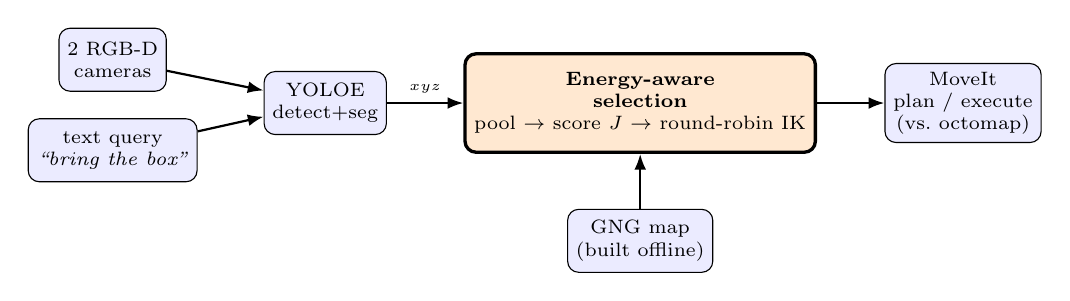
\begin{tikzpicture}[
      font=\scriptsize,
      b/.style={draw, rounded corners, align=center, minimum height=0.8cm,
                inner sep=3pt, fill=blue!8},
      s/.style={draw, rounded corners, align=center, minimum height=1.25cm,
                minimum width=3.0cm, fill=orange!18, very thick},
      a/.style={-{Latex[length=2mm]}, thick},
    ]
    % perception inputs
    \node[b] (cam) at (0, 0.55) {2 RGB-D\\cameras};
    \node[b] (q)   at (0,-0.60) {text query\\{\itshape ``bring the box''}};
    \node[b] (yol) at (2.7, 0)  {YOLOE\\detect+seg};
    % selection (the contribution)
    \node[s] (sel) at (6.7, 0)  {\textbf{Energy-aware}\\\textbf{selection}\\
                                 {\scriptsize pool $\to$ score $J$ $\to$ round-robin IK}};
    \node[b] (gng) at (6.7,-1.75){GNG map\\{\scriptsize (built offline)}};
    % planning / execution
    \node[b] (mv)  at (10.8, 0) {MoveIt\\plan / execute\\{\scriptsize (vs.\ octomap)}};

    \draw[a] (cam) -- (yol);
    \draw[a] (q)   -- (yol);
    \draw[a] (yol) -- node[above,font=\tiny]{$xyz$} (sel);
    \draw[a] (gng) -- (sel);
    \draw[a] (sel) -- (mv);
  \end{tikzpicture}
  \vspace{0.6em}

  {\footnotesize Perception is an \emph{enabler}; the \textbf{energy-aware selection}
  (orange) is the contribution. Depth from the \emph{same} two cameras builds the
  collision octomap that MoveIt plans against. (Fig.~1, right panel.)}
\end{frame}

% ===================== Perception input: text query =====================
\begin{frame}{Perception input: an open-vocabulary text query}
  \footnotesize
  The operator names the object in free-form text; command / filler words are
  stripped and the remaining noun becomes the YOLOE prompt.
  \begin{columns}[T]
    \begin{column}{0.5\textwidth}
      \textbf{Example queries}
      \begin{itemize}
        \item ``bring the banana''
        \item ``pick up the teddy bear''
        \item ``get me the yellow box''
        \item ``hand me the can''
        \item ``can you fetch the bottle''
      \end{itemize}
    \end{column}
    \begin{column}{0.5\textwidth}
      \textbf{Understood as}
      \begin{itemize}
        \item verbs \emph{bring / get / grab / pick / hand / fetch / take} are
              dropped $\Rightarrow$ object noun remains.
        \item \textbf{colour-aware}: ``yellow box'' $\to$ class \texttt{box}, colour
              \texttt{yellow}.
        \item \textbf{aliases}: ``doll''$=$``teddy bear''; ``tin can''$=$``can''.
      \end{itemize}
    \end{column}
  \end{columns}
  \vspace{0.4em}
  {\scriptsize Enabler only: the query yields the target position that the
  capability map and cost $J$ then act on [Wang2025].}
\end{frame}

% ===================== Slide 6 : GNG capability map =====================
\begin{frame}{Base-aware GNG capability map}
  \begin{columns}[T]
    \begin{column}{0.52\textwidth}
      \footnotesize
      One map per arm; nodes tile the reachable workspace [Fritzke1995].
      \textbf{Each node stores:}

      {\scriptsize
      \begin{tabular}{@{}clc@{}}
        \toprule
        Sym. & Contents & Dim. \\
        \midrule
        $x$ & end-effector position (task part) & 3 \\
        $q$ & full 8-DOF config $[d,\theta,q_1\ldots q_6]$ \;\textbf{(IK seed)} & 8 \\
        $w$ & manipulability $\sqrt{\det(JJ^{\top})}$ & 1 \\
        $h$ & holding cost $\lVert$gravity torque$\rVert$ & 1 \\
        \bottomrule
      \end{tabular}}
      \vspace{0.3em}

      \begin{itemize}
        \item BMU search uses $x$ (tile workspace); $q$ is a ready IK seed ---
              config \emph{and} rail, not only quality values.
        \item Rail DOF $(d,\theta)$ sampled $\Rightarrow$ map captures reach that
              \textbf{base motion} adds.
        \item Boundary shell \emph{pinned} to the true reach surface.
      \end{itemize}
    \end{column}
    \begin{column}{0.48\textwidth}
      \centering
      % TODO: Fig. 4 -- GNG node cloud in RViz coloured by manipulability
      \figorbox{figs/fig4_gng_map.png}{5.2cm}{5.0cm}{Fig.~4: GNG map coloured by manipulability, pinned boundary shell \\ TODO: add asset}
    \end{column}
  \end{columns}
\end{frame}

% ===================== Manipulability =====================
\begin{frame}{Manipulability: how dexterous is a posture?}
  \begin{equation*}
    w \;=\; \sqrt{\det\!\left(J J^{\top}\right)}
    \qquad\text{[Yoshikawa1985]}
  \end{equation*}
  \vspace{-0.3em}
  \begin{columns}[T]
    \begin{column}{0.58\textwidth}
      \footnotesize
      \begin{itemize}
        \item $J$ --- the arm's \textbf{Jacobian} at $q$: $\dot{x}=J\dot{q}$
              (here $6\times 8$: 6-DOF pose, 8-DOF chain).
        \item $J J^{\top}$ collapses the rectangular $J$ into a $6\times6$ matrix
              we can take a determinant of.
        \item $w$ is the \textbf{volume of the manipulability ellipsoid}
              ($w=\sigma_1\cdots\sigma_6$, the singular values of $J$).
      \end{itemize}
      \vspace{0.2em}
      \begin{itemize}
        \item[\textcolor{red!70!black}{$\blacksquare$}] \textbf{large $w$}: round
              ellipsoid --- moves easily in any direction.
        \item[\textcolor{blue!70!black}{$\blacksquare$}] \textbf{small $w\!\to\!0$}:
              collapsed --- near a \textbf{singularity}, IK ill-conditioned.
      \end{itemize}
    \end{column}
    \begin{column}{0.42\textwidth}
      \centering
      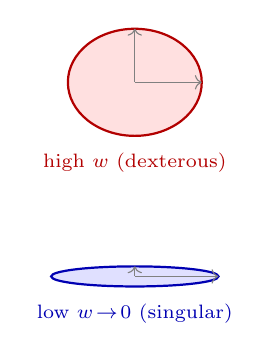
\begin{tikzpicture}[scale=0.85]
        \begin{scope}[shift={(0,1.0)}]
          \draw[fill=red!12,draw=red!70!black,thick] (0,0) ellipse (1.0 and 0.8);
          \draw[->,gray] (0,0) -- (1.0,0);  \draw[->,gray] (0,0) -- (0,0.8);
          \node[red!70!black,font=\scriptsize] at (0,-1.2){high $w$ (dexterous)};
        \end{scope}
        \begin{scope}[shift={(0,-1.9)}]
          \draw[fill=blue!12,draw=blue!70!black,thick] (0,0) ellipse (1.25 and 0.15);
          \draw[->,gray] (0,0) -- (1.25,0); \draw[->,gray] (0,0) -- (0,0.15);
          \node[blue!70!black,font=\scriptsize] at (0,-0.55){low $w\!\to\!0$ (singular)};
        \end{scope}
      \end{tikzpicture}
    \end{column}
  \end{columns}
  \vspace{0.3em}
  \hrule height 0.3pt \vspace{0.3em}
  {\footnotesize \textbf{In this work:} $w$ is a per-node map layer (Fig.~4) and
  enters cost $J$ with a \emph{minus} sign, so a more dexterous candidate scores
  cheaper.}
\end{frame}

% ===================== Slide 7 : Energy cost J =====================
\begin{frame}{Energy cost $J$}
  \small
  \[
    J = w_{gl}\frac{\Delta_{\mathrm{lin}}}{\rho_{gl}}
      + w_{gr}\frac{\Delta_{\mathrm{rot}}}{\rho_{gr}}
      + w_{arm}\frac{\Delta_{\mathrm{arm}}}{\rho_{arm}}
      + w_{dist}\frac{e}{\rho_{dist}}
      + w_{hold}\frac{h}{\rho_{hold}}
      - w_{manip}\frac{m}{\rho_{manip}}
  \]
  \begin{columns}[T]
    \begin{column}{0.46\textwidth}
      \footnotesize
      \begin{itemize}
        \item Rail-linear, rail-rotation, arm travel; tool-to-object distance $e$;
              holding torque $h$; $-$manipulability $m$.
        \item Rail linear \& rotation carry \emph{separate} weights (metres vs
              radians of a heavy carriage).
        \item Each term $\div\,\rho$ (median over calibration picks) $\Rightarrow$
              dimensionless; a weight reads as a priority.
        \item Proxy for pick energy --- not exact energy; validated against
              measured trajectory energy [EnergySLR2024].
      \end{itemize}
    \end{column}
    \begin{column}{0.54\textwidth}
      \centering
      \scriptsize
      \begin{tabular}{@{}llrr@{}}
        \toprule
        Term & Symbol & Weight & Ref.\ $\rho$ \\
        \midrule
        Rail linear travel      & $\Delta_{\mathrm{lin}}$ & 2  & 0.95  \\
        Rail rotation travel     & $\Delta_{\mathrm{rot}}$ & 12 & 0.70  \\
        Arm joint travel         & $\Delta_{\mathrm{arm}}$ & 20 & 6.00  \\
        Tool-to-object distance  & $e$                     & 3  & 1.36  \\
        Gravity holding torque   & $h$                     & 1  & 2.90  \\
        Manipulability (subtr.)  & $m$                     & 1  & 0.145 \\
        \bottomrule
      \end{tabular}
      \\[3pt]
      {\scriptsize Table 1. Calibrated weights and references for $J$.}
    \end{column}
  \end{columns}
\end{frame}

% ===================== Selection: pooling + round-robin =====================
\begin{frame}{Selection: pooling and round-robin search}
  \begin{columns}[T]
    \begin{column}{0.5\textwidth}
      \footnotesize
      \begin{enumerate}
        \item \textbf{Pool} --- gather map nodes within a radius of the object,
              from \emph{both} arms' maps (the reachability filter).
        \item \textbf{Score} every candidate by $J$; both arms compared on one scale.
        \item \textbf{Round-robin} --- interleave the two arms so one cannot consume
              every attempt; lowest-$J$ arm gets a small head start.
        \item \textbf{Plan-only} --- seed IK from the node, ask MoveIt for a
              collision-free plan; the arm never moves during the search.
        \item \textbf{First valid plan wins} --- only that candidate is executed;
              on abort, fall through to the next.
      \end{enumerate}
    \end{column}
    \begin{column}{0.5\textwidth}
      \centering
      % TODO: Fig. 5 -- top-view energy-selection illustration (values from logged pick)
      \figorbox{figs/fig5_selection.png}{5.2cm}{5.0cm}{Fig.~5: $J$ picks the cheaper arm/base (may not be the nearest) \\ TODO: add asset}
    \end{column}
  \end{columns}
\end{frame}

% ===================== Slide 8 : Results =====================
\begin{frame}{Results (NVIDIA Isaac Sim)}
  \begin{columns}[T]
    \begin{column}{0.52\textwidth}
      \begin{itemize}
        \item[(a)] Treating the rail as a DOF enlarges the reachable workspace
              \textbf{$\sim$5.1$\times$} vs.\ an arm-only baseline (E1).
        \item[(b)] GNG-seeded IK: success $\uparrow$, solve-time $\downarrow$ ---
              \textbf{[results pending]}.
        \item[(c)] Energy-aware vs.\ nearest / fixed / random: base travel and
              mechanical energy --- \textbf{[results pending]}.
      \end{itemize}
      \vfill
      {\footnotesize All numbers come from Isaac Sim; physical validation is future
      work.}
    \end{column}
    \begin{column}{0.48\textwidth}
      \centering
      % TODO: Fig. 6 -- (a) workspace-gain bar (ready); (b) energy boxplot (pending E3)
      \figorbox{figs/fig6_results.png}{5.2cm}{5.0cm}{Fig.~6: (a) workspace gain $\sim$5.1$\times$ | (b) energy vs.\ baselines [pending] \\ TODO: add asset}
    \end{column}
  \end{columns}
\end{frame}

% ===================== Slide 9 : Future work =====================
\begin{frame}{Future work}
  The map + energy cost $J$ extend naturally along several directions:
  \vspace{0.3em}
  \begin{itemize}\footnotesize
    \item \textbf{Dual-arm collaboration.} Use \emph{both} arms together --- for
          heavy objects or carrying more than one item at once --- scored on the
          same shared-base energy cost [DAGPlan2024, RoboPARA2025].
    \item \textbf{Object hand-over.} Deliver to a person (the ``hand things to the
          people'' goal of the intro), and \emph{arm-to-arm} hand-over whose
          transfer point is chosen by the same cost $J$.
    \item \textbf{Human--robot interaction.} Read human pose / pointing gestures to
          disambiguate \emph{which} object is wanted, and to reach around people
          safely [Lisondra2025].
    \item \textbf{Contact-based grasping.} Move from the current approach-only,
          plan-only search to real grasp execution (contact, close, lift) with
          regrasp on failure.
    \item \textbf{Energy-aware multi-pick sequencing.} Extend $J$ from one action
          to a \emph{sequence} of picks, planning an energy-optimal base-pose order
          [BaSeNet2024].
  \end{itemize}
\end{frame}

% ===================== Toward real-world deployment =====================
\begin{frame}{Toward real-world deployment}
  \begin{itemize}
    \item \textbf{The platform already exists.} Four Kinova Gen3 Lite arms, a
          Modbus-driven ceiling gantry, and a Livox Mid360 LIDAR --- driven from
          the \emph{same} URDF used in simulation.
    \item \textbf{Direct energy validation.} Measure real rail + arm motor
          current / power to confirm that minimizing $J$ lowers \emph{measured}
          energy --- backing the ``Energy-Aware'' claim beyond the simulated proxy.
    \item \textbf{Perception likely improves.} YOLOE is trained on natural images,
          so real RGB-D should be \emph{more} reliable than synthetic Isaac renders.
    \item \textbf{Open gaps.} Heavy-rail dynamics and friction, kinematic
          calibration, and safety while sharing space with people.
  \end{itemize}
\end{frame}

% ===================== Slide 10 : Conclusion =====================
\begin{frame}{Conclusion}
  \begin{itemize}
    \item \textbf{Contributions:}
      \begin{itemize}
        \item Energy cost $J$ that selects the arm \emph{and} the full 8-DOF
              configuration together (rail travel included).
        \item A base-aware GNG capability map: per-node IK seed, manipulability,
              and holding cost, with a pinned boundary shell.
        \item Evaluation in Isaac Sim vs.\ nearest / fixed / random baselines.
      \end{itemize}
    \item Treating the ceiling rail as a real DOF pays off: \textbf{$\sim$5.1$\times$}
          larger reachable workspace.
    \item \textbf{Sim-only} here $\to$ hardware validation on the physical platform
          is left for future work.
  \end{itemize}
  \vfill
  \centering \Large Thank you --- questions?
\end{frame}

% ===================== References =====================
\begin{frame}[allowframebreaks]{Selected references}
  \scriptsize
  \setbeamertemplate{bibliography item}[text]
  \begin{thebibliography}{99}
    \bibitem{Zacharias2007} F. Zacharias, C. Borst, G. Hirzinger,
      ``Capturing robot workspace structure: representing robot capabilities,''
      \emph{IEEE/RSJ IROS}, 2007.
    \bibitem{Yoshikawa1985} T. Yoshikawa, ``Manipulability of Robotic Mechanisms,''
      \emph{Int. J. Robotics Research}, 4(2), 1985.
    \bibitem{Fritzke1995} B. Fritzke, ``A Growing Neural Gas Network Learns
      Topologies,'' \emph{NIPS 7}, 1995.
    \bibitem{Makhal2018} A. Makhal, A. K. Goins, ``Reuleaux: Robot Base Placement
      by Reachability Analysis,'' \emph{IEEE IRC}, 2018.
    \bibitem{RM4D2024} M. Rudorfer, ``RM4D: A Combined Reachability and Inverse
      Reachability Map \ldots{} by Dimensionality Reduction to 4D,'' arXiv:2410.06968.
    \bibitem{MoMaPos2024} B. Shao \emph{et al.}, ``MoMa-Pos: \ldots{} Base Placement
      Optimization for Mobile Manipulation,'' arXiv:2403.19940.
    \bibitem{BaSeNet2024} L. Naik \emph{et al.}, ``BaSeNet: \ldots{} Base Pose
      Sequence Planning for Pickup Tasks,'' \emph{IEEE/RSJ IROS}, 2024.
    \bibitem{InvReach2022} T. Sandakalum, N. X. Yao, M. H. Ang, ``Inv-Reach Net:
      Deciding mobile platform placement for a given task,'' \emph{Humanoids}, 2022.
    \bibitem{IKDiffuser2025} Z. Zhang, Z. Jiao, ``IKDiffuser: A Diffusion-based
      Generative Inverse Kinematics Solver \ldots,'' arXiv:2506.13087.
    \bibitem{DAGPlan2024} Z. Gao \emph{et al.}, ``DAG-Plan: \ldots{} Dual-Arm
      Cooperative Planning,'' arXiv:2406.09953.
    \bibitem{RoboPARA2025} S. Duan \emph{et al.}, ``RoboPARA: Dual-Arm Robot
      Planning with Parallel Allocation and Recomposition,'' arXiv:2506.06683.
    \bibitem{Wang2025} A. Wang \emph{et al.}, ``YOLOE: Real-Time Seeing Anything,''
      \emph{ICCV}, 2025.
    \bibitem{EnergySLR2024} A. Gupta, ``Energy Efficiency in Robotics Software:
      A Systematic Literature Review,'' arXiv:2508.12170.
    \bibitem{IsaacSim2026} S. Gao \emph{et al.}, ``NVIDIA Isaac Sim: \ldots{}
      GPU-Accelerated Simulation for Robotics,'' arXiv:2606.03551.
    \bibitem{Coleman2014} D. Coleman \emph{et al.}, ``Reducing the Barrier to Entry
      \ldots{}: a MoveIt! Case Study,'' arXiv:1404.3785.
    \bibitem{Carpentier2019} J. Carpentier \emph{et al.}, ``The Pinocchio C++
      library,'' \emph{IEEE/SICE SII}, 2019.
    \bibitem{Lisondra2025} M. Lisondra \emph{et al.}, ``Embodied AI with Foundation
      Models for Mobile Service Robots: A Systematic Review,'' arXiv:2505.20503.
    \bibitem{Jayathilaka2025} W. A. D. M. Jayathilaka \emph{et al.}, ``A Novel Hybrid
      Robot Configuration for Enhanced Accessibility and Space Efficiency,''
      Springer, 2025.
  \end{thebibliography}
\end{frame}

\end{document}
